\renewcommand*{\thesection}{\arabic{section}.}

\chapter{Real Organisms and the Choice of Kinetic Systems}
\markboth{REAL ORGANISMS}{}

In the introduction it was stated that a major aim would be to provide a suitable theoretical framework, in which to consider how variability in an organism at the genetic (or information storage) level will be expressed at the level of measurements made on the `system' which is the organism. The purpose of this chapter is to show precisely what is meant by this, to provide such a framework, to consider properties of unimolecular systems in relation to it and finally to introduce a number of general concepts in connection with these systems. In Chapter II consideration will be given to the formulation, within this scheme, of more complex metabolic systems which can more reasonably stand as analogues for real organisms.

Before proceeding to consider specific types of systems it is important to make clear the general point of view which is to be adopted. Genes act by specifying the precise properties of functional units, usually proteins, which themselves act in many cases by catalysing specific reactions within a metabolic network of some sort. Accordingly many aspects of the general gene-action problem will be reflected in a more limited and abstract problem, namely that of how enzymes interact within a multi-enzyme system to determine measurable properties of the system, as for example the concentration of a given metabolite or the metabolic flux at a point in the network. Whilst no apology will be made for this abstraction from the general problem, the genetic systems to which the limited treatment is most relevant will clearly be simple unicellular or synctial organisms growing in a well defined culture medium. For complex multicellular organisms in a complex environment it will be less obviously relevant, although even here it may be applicable to the more biochemical type of character.

Given then that a first attempt to understand something of the quantitative aspects of gene action may be reasonably limited to a consideration of multi-enzyme systems, two further tactical questions arise. The first of these is concerned with the quantitative importance of the spatial organisation of metabolism within the cell. There is ample evidence that such organisation occurs, as for example at the high level of cell organelles such as mitochondria, and, at a lower level, where it has been suggested that several enzymes in a pathway are physically associated in a particle (Wagner and Bergquist, 1963) thus promoting the passage of substrates from one enzyme molecule to another. However, there is reason to suppose that this organisation, whilst certainly important, is not absolutely crucial to the cell metabolism. Evidence for this is that mutants which block the production of various intermediates can be completely relieved by relatively low concentrations of the intermediate in the external medium. Whilst in principle it would be desirable to include spatial organisation in a treatment of multi-enzyme systems, this would be impossibly difficult, both because of a lack of reliable information about spatial organisation and because it would involve considering chemical concentration as dependent on position and subject to diffusion equations, a great extension of an already complex problem. Certainly, if we have to compromise between either a multi-enzyme system containing many enzymes related by a specific transformational and control diagram, but neglecting spatial organisation, or a system containing only a few enzymes and allowing for spatial organisation, the first alteṛative must be taken. This is because gene action and interaction are likely to depend crucially on the fact that the `points of action' of the different genes are embedded in a metabolic network. To dispense with this network would thus be seriously to distort the very aspect of the system which is under consideration, that is gene action.

The second tactical question is concerned with the relative importance to be attached to what might be called the ``long term'' and the ``transient'' behaviour of multi-enzyme systems. A general `open' multi-enzyme is represented below. This exists within a fixed volume and allows passage of metabolites between the surrounding medium and the inner `metabolic space', across the surface of the volume.

\centerline{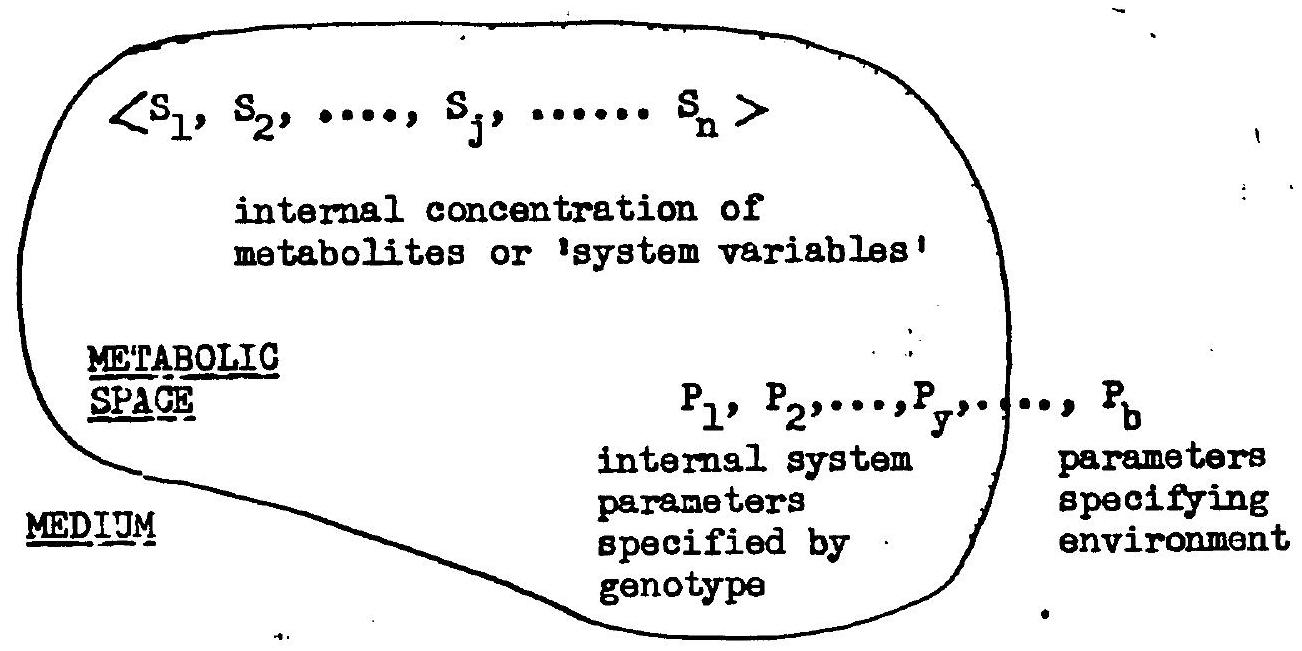
\includegraphics[scale=0.26]{2023_01_30_a974a42f7b7381f3f940g-025}}

The surrounding space is assumed to be sufficiently large and well mixed that concentrations of metabolites in it can be considered as constants in the `environment' of the metabolising volume. Since perfect mixing is also assumed internally the state of the system will be specified at any moment by the instantaneous molar concentrations $\left(S_{1}, \ldots S_{n}\right)$ ) of the $n$ variable metabolites. These, together with the fixed parameters $\left(P_{1}, \ldots P_{b}\right)$, determine the change which will ensue in the system at the next moment. This situation is expressed mathematically by saying that the `equations of motion' for the system are the set of $n$ 1st ordinary differential equations (D.E.).
%
\begin{equation}
\frac{d\left(S_{i}\right)}{d t} = \dot{S}_{i}=\varphi_{i}\left(S_{1}, \ldots \ldots, S_{n}, P_{1}, \ldots \ldots, P_{b}\right)
\label{eqn:11}
\end{equation}
%
The parameters $P$ include the constant concentration of environmental metabolites, kinetic constants belonging to genetically defined proteins, and other determinants such as the volume and surface area of the metabolising space. For the present the precise nature of the nonlinear functions $\varphi_{i}(\ldots$) may be left open, although it is clear that they will depend on expressions giving the instantaneous rates of the various metabolic transformation both within the system and across its surface. The respective contributions of genotype and environment to the properties of an organism are thus represented in the abstract problem as the way in which the solution of \eqref{eqn:11} depends on $P_{1}, P_{2}, \cdots, P_{b}$.

`Long term' means that interest is primarily in the solution of \eqref{eqn:11} a long time after its release from initial conditions $S_{i}^{0}$. Such a solution may approach a stationary steady state, when a set of values $S_i$ arise such that all the $\dot{S_i}$ become zero, or alternatively, a steady-state, in with the $S_{i}$ arise such that $S_{i}$ do not become time independent but a trajectory arises such that the system repeats its motion at regular intervals, $T$, satisfying the conditions
%
$$ \int_\alpha^{\alpha + T} \dot{S}_i dt = 0 $$
%
where $\alpha$ is an arbitrary large time. Such steady state trajectories are clearly completely characterised if the values of the $S_{i}$ are known at just one point on the trajectory. A third possible long term solution is one which is neither stationary nor steady state.

It seems clear, in the context of this discussion, that attention should be concentrated on the long term solutions \eqref{eqn:11}. Such solutions do not depend precisely on arbitrary initial conditions, but only on the system's genetically specified set of proteins together with the concentration of chemicals external to the system. If there are alternative solutions the $S_{i}^{0}$ will determine which one is reached. In principle the way is now clear to study the dependence of the long term solutions of \eqref{eqn:11} on the parameters $P_{1}, P_{2}, \ldots$, such dependence being representative of the more general dependence of the phenotype on the genotype and the environment for real genetic systems (organisms).

\section{Evaluating the stationary state}

In practice, however, even such abstract studies cannot be carried out by mathematical manipulation of \eqref{eqn:11} but, owing to the large number of system variables $S_{i}$ and the non-linearity of the functions $\varphi_{i}(\hspace{2pt})$, must be done numerically with the aid of a computer only on the simplest assumptions, namely that all $\varphi_{i}(\hspace{2pt})$ are linear functions of the $S_{i}$, can an explicit algebraic stationary steady state solution of \eqref{eqn:11} be obtained and such linear models, whilst of considerable interest, do not properly allow for basic aspects of metabolic organisation like bimolecularity and feedback inhibition.

With regard to obtaining the long term solution of \eqref{eqn:11} by numerical means and for specific values of the parameters $P_{1}, P_{2} \ldots$, there are two distinct situations, that in which the solution is a stationary one, and that where it is a non-stationary steady state or limit cycle. In both cases our interest lies not only in the solution but also in the response or sensitivity of this solution to the parameters P, that is in the influence of variation of genotype and environment on the phenotype. This response will appear naturally in the form of a matrix since it is the response of the phenotype, represented by a group of measurements on the system, to the genotype represented by a group of system parameters.

For the case of a system possessing a stationary solution the equations to be solved are, from \eqref{eqn:11}, the $n$ non-linear simultaneous equations
%
\begin{equation}
\varphi_{i}\left(S_{1}, S_{2}, \ldots, P_{1}, P_{2}, \ldots \right)=0
\label{eqn:12}
\end{equation}
%
Suppose we possess a concentration vector $S_{i}$ such that each equation differs from zero by only a small deviation $d_{i}$ then
%
\begin{equation}
d_{i} = \varphi_{i}\left(S_{1}, S_{2} \ldots\right)
\label{eqn:13}
\end{equation}
%
The problem of finding the stationary solution $\olsi{S}_{i}$ is that of how to adjust the $S_{i}$ in \eqref{eqn:13} so that all $d_{i}$ approach zero.

Let $\delta S_{i}$ be the necessary adjustment to $S_{i}$ so that $\olsi{S}_{i} = S_{i} + \delta S_{i}$. Now, since $\olsi{S}_{i}$ is the exact solution, $\varphi_{i}\left(\olsi{S}_{1}, \olsi{S}_{2}, \ldots\right.)=0$

or
%
$$
\varphi_{i}\left(S_{1} + \delta S_{1}, S_{2} + \delta {S_{2}}, \ldots \right) = 0
$$
%
which, ignoring terms above 1st degree in a Taylor expansion, gives
%
$$
\varphi_{1}\left(S_{1}, S_{2}, \ldots\right) + \sum_{j=1,n} \frac{\partial \varphi_{i}}{\partial S_{j}} \times \delta S_{j}=0
$$
%
In vector and matrix notation and using (1.3) this becomes
%
\begin{equation}
d_{i} \bumpeq \left[\frac{\partial d_{i}}{\partial S_{j}}\right] \cdot \delta S_{j}
\label{eqn:14}
\end{equation}
%
An approximate $\delta S_{i}$ is thus given by solving \eqref{eqn:14}
%
\begin{equation}
\delta S_{j} = -\left[\frac{\partial d_{i}}{\partial S_{j}}\right]^{-1} \cdot d_{i}
\label{eqn:15}
\end{equation}
%
The numerical solution of \eqref{eqn:12} then consists in progressively correcting the existing $S_{1}$ using \eqref{eqn:13} and \eqref{eqn:15} until the deviations $d_{i}$ are sufficiently close to zero. This `iterative' process will be returned to in CH. IV when the numerical and computer aspects will be discussed.

The matrix $\left[\frac{\partial d_{i}}{\partial S_{j}}\right]$ or $\left[\frac{\partial \varphi_{i}}{\partial S_{j}}\right]$, evaluated at the stationary solution, is also involved in finding the sensitivity of this solution to small changes in $P_{1}, P_{2}$, etc. In this case if the original solution was $\olsi{S}_{i}$ the new solution, $\olsi{S}_{i} + \delta \olsi{S}_{i}$ is one corresponding to, say, the change $P_{1} \rightarrow P_{1} + \delta P_{1}$, and we have the stationary condition \eqref{eqn:12} to satisfy for both the old and the new solution.
%
$$ \mbox{Thus } \psi_{i}\left(\olsi{S}_{1}, \olsi{S}_{2}, \ldots, P_{1}, P_{2}, P_{3} \ldots\right)=0, \text { for } 1=1 \text { to } N $$
\vspace{-6pt}
$$ \mbox{and also } \psi_{i}\left(\olsi{S}_{1}+\delta \olsi{S}_{1}, \olsi{S}_{2}+\delta \olsi{S}_{2}, \ldots P_{1}+\delta P_{1}, P_{2}, P_{3}\right)=0, \text { for } i=1 \text{ to } N $$
%
\vspace{14pt}
Using these two conditions and assuming $\delta \mathrm{P}_{1}$ sufficiently small for higher terms in the Taylor expansion to be ignored we get
%
$$ \frac{\partial \varphi_{i}}{\partial P_{1}} \cdot \delta P_{1} + \sum \frac{\partial \varphi_{i}}{\partial S_{j}} \cdot \delta \olsi{S}_{j}=0 $$
%
\begin{equation}
\frac{\delta \olsi{S}_{i}}{\delta P_{1}} = -\left[\frac{\partial \varphi_{i}}{\partial S_{j}}\right]^{-1} \cdot \frac{\partial \varphi_{i}}{\partial P_{1}}
\label{eqn:16}
\end{equation}

%
The relation \eqref{eqn:16} shows how stationary values of the system variables $\olsi{S}_{i}$ will respond to a small change in a parameter and can be used as a basis for considering how a general phenotype `measure' made on a stationary system will respond. Such a measure, which reflects one aspect of the phenotype, is conceived as being the result, $\olsi{M}$, of a particular measuring operation carried out upon the stationary system. $\olsi{M}$ will depend upon the variables defining the stationary state and possibly some system parameters so that in general
%
\begin{equation}
\overline{M}=\olsi{M}\left(\olsi{S}_{1}, \ldots \olsi{S}_{n}, P_{1}, \ldots P_{b}\right)
\label{eqn:17}
\end{equation}
%
Here the notation $\olsi{\mathrm{M}}(\ldots)$ merely spans, the ``function of certain arguments, whose value is $\olsi{M}$''. The response of $\olsi{M}$ to a particular parameter, say $P_{1}$, is conveniently defined as the `sensitivity coefficient' $C_{P_{1}}^{\olsi{M}}$ which compares the fractional response in $\olsi{M}$ to the small fractional disturbance in $P_{1}$ which produced it. This concept is developed further in CH. III but for the moment we can write
%
$$ C^{\olsi{M}}_{P_1} = \frac{P_1}{\olsi{M}} \frac{\partial \olsi{M}}{\partial P_1} $$
%
Using \eqref{eqn:16} and \eqref{eqn:17} we therefore get
%
\begin{equation}
\mathrm{C}_{P_1}^{\olsi{M}} = \frac{1}{\olsi{M}} \frac{\partial M}{\partial \olsi{S}_{j}} \times\left[\frac{\partial \varphi_{i}}{\partial S_{j}}\right]^{-1} \times P_{1} \frac{\partial \varphi_{i}}{\partial P_{1}}
\label{eqn:18}
\end{equation}
%
More generally the phenotype is described by a group of such measures $\olsi{M}_{1}, \ldots, \olsi{M}_{x}, \ldots \olsi{M}_{a}$ and the genotype and environment by a group of system parameters subject to variation $P_{1}, \ldots, P_{y}, \ldots, P_{b}$. The sensitivity of the phenotype to the genotype and the environment will then be displayed in the matrix of coefficients $\left[C_{P_{y}}^{\olsi{M_{X}}}\right]$, where
%
\begin{equation}
\left[C_{P_{y}}^{\olsi{M}_{X}} \right]=\left[\frac{1}{\olsi{M}_{X}} \frac{\partial \olsi{M}_{X}}{\partial \olsi{S}_{j}}\right] \times\left[\frac{\partial \varphi_{i}}{\partial S_{j}}\right]^{-1}  \times\left[P_{y} \frac{\partial \varphi_{j}}{\partial P_{y}}\right]
\label{eqn:19}
\end{equation}
%
The matrix $\left[\frac{\partial \varphi_{i}}{\partial S_{j}}\right]$ which appears in \eqref{eqn:17} and \eqref{eqn:19} is in fact also the matrix which underlies the dynamical behaviour of the system when close to the stationary state.

Thus suppose the system to be close to a stationary state so that $S_{i}=\olsi{S}_{i} + X_{i}$ where $X_{i}$ is small. Inserting this in \eqref{eqn:11} and ignoring terms above 1st order in the expansion we get
%
\begin{equation}
\dot{X}_{j} = \left[\frac{\partial \varphi_{i}}{\partial S_{j}}\right]_{S_{j}=\olsi{S}_{j}} \times X_{j}
\label{eqn:110}
\end{equation}
%
thus the `dynamical matrix', $D$, of the system is just $\left[\frac{\partial \varphi_{i}}{\partial S_{j}}\right]_{S_{j}=\olsi{S}_{j}}$.

The stability or otherwise of the stationary solution will then depend on whether the `eigenvalues' of $D$ all have negative real parts.

\section{The limit cycle}

Can similar techniques be used when a system does not possess a stationary steady state? Let us consider a system possessing a limit cycle type of `long term' solution, when it may be possible to use such a technique. Suppose that we have a trajectory close to an exact solution and defined by a concentration vector $S_{i}$ and period $T$ then the deviations defined by
%
\begin{equation}
d_{i}=\int_{t}^{t+T} \varphi_{1}\left(S_{1}, S_{2}, \cdots \cdot\right) \cdot dt
\label{eqn:111}
\end{equation}
%
correspond to the deviations of \eqref{eqn:13} in the stationary case. The integration referred to in  \eqref{eqn:111} is performed on the set of D.E. \eqref{eqn:11}, starting at time $t$ with the proposed vector $S_{i}$. The meaning of these residues is illustrated below.

\begin{center}
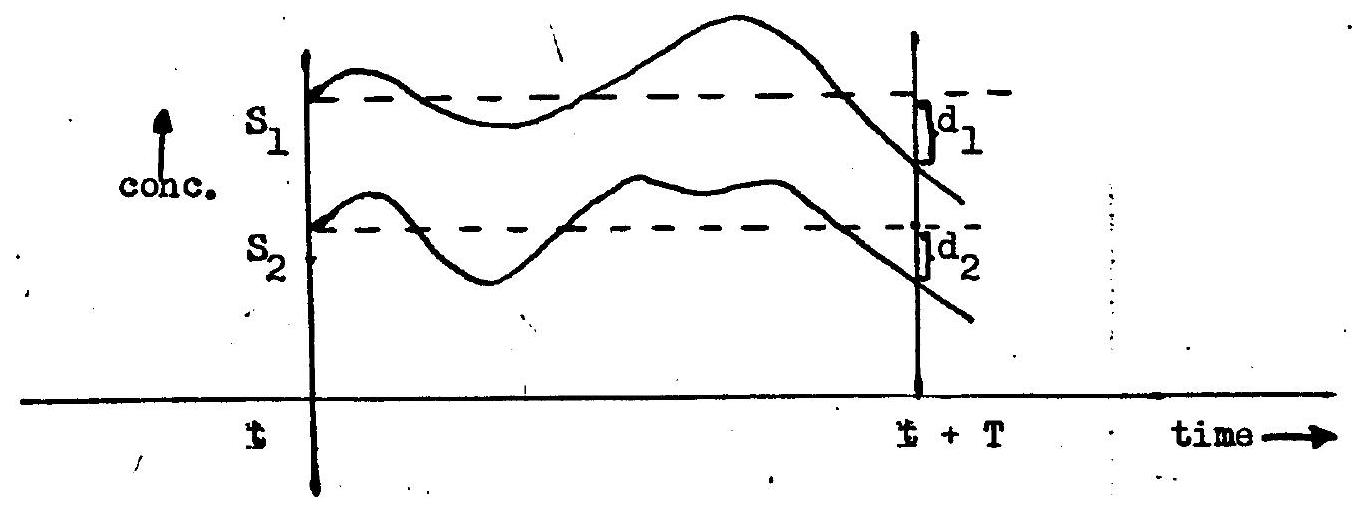
\includegraphics[max width=\textwidth]{2023_01_30_a974a42f7b7381f3f940g-033}
\end{center}

The problem of finding an exact solution is, as before, to manipulate the approximate solution until the $d_{i}$ are sufficiently close to zero. This can be done by adjusting all but one of the $S_{i}$ and also the approximate period $T$, parameters which can be designated $\xi_1$ to $\xi_n$. The holding constant of one of the $S_{i}$ merely serves to define the arbitrary time, $t$, which is being used to characterise the final limit cycle. The small corrections to be applied to the existing values of the parameters are calculated by the relation
%
\begin{equation}
\delta \xi_{j} = -d_{i} \bigg/\left[\frac{\partial d_{i}}{\partial \xi_{j}}\right]
\label{eqn:112}
\end{equation}
%
which is analogous to relation \eqref{eqn:15}, and a similar `iteration' is performed using \eqref{eqn:112} and  \eqref{eqn:111}. The matrix $\left[\frac{\partial d_{i}}{\partial \xi_{j}}\right]$ can, as before, also be used to discover the sensitivity of measures connected with the limit cycle to the parameters $P_1, P_2, \cdots P_b$.

There is, however, an important practical difference between the two cases just discussed in that the evaluation of the $d_i$ for the limit cycle case involves, even on the best assumptions, many hundreds of times more computer operations than does the stationary case. This is because the integration of the system of D.E. \eqref{eqn:11} over the period $T$ involves many hundreds of evaluations of the $S_i$, each of which corresponds to one $d_i$ evaluation in the stationary state computation.

If the period $T$ is large or the equations difficult to integrate the factor may be even worse and the difficulty is further compounded by the requirement that the $d_i$ have to be calculated to a high accuracy if the numerical differentiation involved in estimating the matrix $\left[\frac{\partial d_i}{\partial \xi_j}\right]$ of \eqref{eqn:112} is to be reliable. It appears, therefore, that whilst the stationary type of computation proves quite feasible for reasonably large networks, say less than forty enzymes, it becomes totally impracticable for networks having limit cycle solutions. This conclusion applies a fortiori to systems whose `long term' solution, although regular in some sense, cannot be described by limit cycles. In these circumstances, remembering that an interact in gene action involves networks of some size and complexity, consideration can only be given to systems possessing stable stationary state solutions. This limitation seems unavoidable, whether it turns out to be serious will depend on how frequently non stationary long term behaviour is encountered in metabolic systems under study.

\section{The use of rate equations}

Accepting then the considerable simplification that only stationary solutions of homogeneous multi-enzyme systems will be considered it is hoped that such solutions will still represent important. aspects of the genotype-phenotype relation. This hope rests mainly on the strategy that minimal compromise will subsequently be made in representing the structure of metabolic networks, the structure clearly being critical to any attempt at representing gene-action.

The nature of the system variables $S_{i}$ has deliberately been left open until this point. A reasonably complete set of such variables for a metabolic system has usually been taken as a set of concentrations of intermediary metabolites together with a set of concentrations of enzymic intermediates. The set of dynamical functions $\varphi$ (..) are then written down, using the `Guldberg-Waage' law of mass-action, and used as a basis for further analysis, as for example in Pring (1967).

However, when interest is centred, as here, on the properties of the stationary state it is possible to avoid considering enzymic intermediates by using the fact that when the complete system is at a stationary state so will be the enzymic intermediates belonging to each enzyme. The `net flux' carried by each enzyme at the stationary state will then be given by the King-Altman rate expression of steady state enzyme kinetics as discussed in the introduction. Thus the number of system variables is reduced to the number of intermediary metabolites and expressions $\varphi_{i}(\ldots)$ for their rates of change become sums and differences of rate expressions. The expressions $\varphi_{i}$ (\ldots) made up

\bigskip
\centerline{\bf\large General theoretical aspects of multi-enzyme systems}

\begin{center}
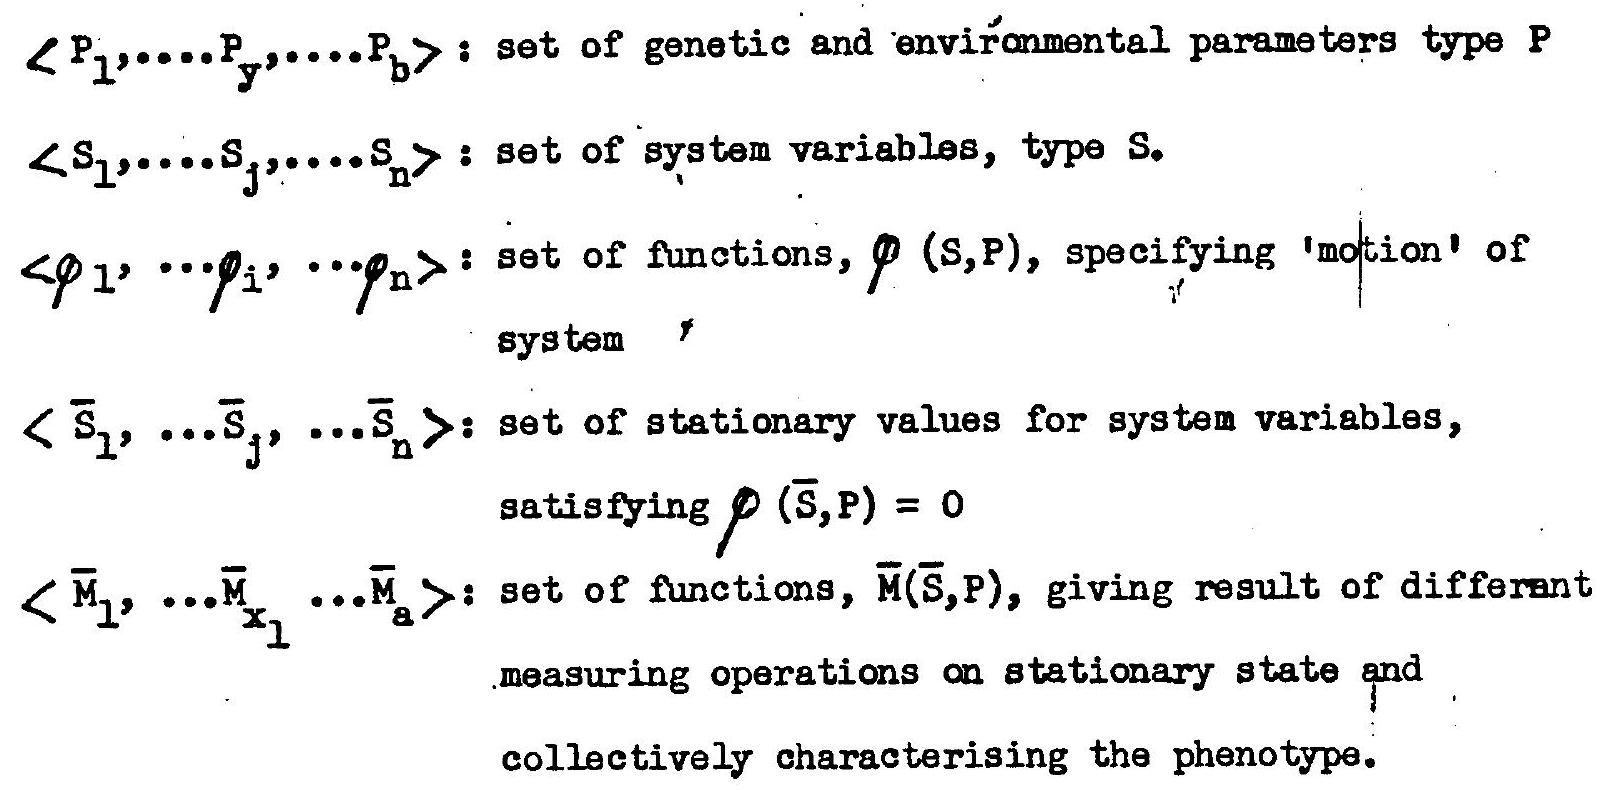
\includegraphics[max width=\textwidth]{2023_01_30_a974a42f7b7381f3f940g-036}
\end{center}

\pagebreak
\centerline{\bf\large Numerical operations}

i) Evaluate matrix $\left[D'\right]=\left[\frac{\partial \varphi_{i}}{\partial S_{j}}\right]$ at present values of $S_{j}$ by numerical approximation.

ii) Use it to find $\olsi{S}$ by means of the `iteration'

$$
\begin{aligned}
\mbox{1: } & \delta S_{j} = \left[D^{\prime}\right]^{-1} \cdot \varphi_{i} \\
& S_{j} \leftarrow S_{j} + \delta S_{j} \\
& \rightarrow \mbox{(goto) } 1 \text { unless all } \varphi_{i} \bumpeq 0
\end{aligned}
$$

Having thus obtained $\olsi{S}$ and $D=\left[\frac{\partial \varphi_{i}}{\partial {S_{j}}}_{\mbox{at }S=\olsi{S}}\right]$

iii) Compute the phenotype/genotype, environment) sensitivity matrix using the relation

$$
\left[
C_{P_y}^{\olsi{M}_X}\right] = \left[\frac{1}{M_X} \frac{\partial M_X}{\partial S_j}\right] \times [D]^{-1} \times\left[\frac{P_y \partial \varphi_i}{\partial P_y}\right]
$$

iv) Characterise the dynamics of the system close to the stationary state by extracting eigenvalues of $\left[ D \right]$.

\noindent\rule{\textwidth}{1pt}

in this way will only approximate to the `true' dynamics of the system, but Pring (1967) has shown that this approximation may be a very good one. However, the stationary state and its properties will not be in any way affected by this simplification and the dimension of a given system will be reduced by a considerable factor. For example a system with 20 metabolites and 25 enzymes each requiring, on the average, 4 enzymic intermediates to describe its kinetics, would have a dimension of 120 system variables. In this case a reduction in dimension of 6 fold would result from the use of rate expressions in making up the functions $\varphi_{i}$ for the 20 intermediate metabolites, properties of the stationary state would be identical with the `true' system and even the dynamics would be a good approximation.

Accordingly, unless otherwise stated, system variables will be taken to be the set of intermediary metabolite concentration. The set of dynamical functions $\varphi_{i}$ attached to them will then be an approximation to the true dynamics, involving the use of rate expressions, which nevertheless leaves the properties of the stationary state unaltered.

Our general theoretical and computational framework for multienzyme systems which possess a stationary solution is now clear. This is summarised on p.14 opposite, where it can be seen that the set of dynamical functions $\varphi_{1}, \ldots ., \varphi_{\mathrm{n}}$ and the matrix $[\mathrm{D}]=\left[\frac{\partial \varphi_{i}}{\partial S_{j}}\right]$ play an important role. The remainder of this chapter will consider the particular situation when the $\varphi_{1}$ represent systems of unimolecular reactions. Chapter II will then be concerned with progressively showing how more general systems, having the necessary realistic detail, may be formulated in terms of suitable sets of functions $\varphi_{i}$, themselves based on rate expressions.

The remainder of this chapter will consider the particular situation when the $\varphi_1$ represent systems of unimolecular reactions. Chapter II will then be concerned with progressively showing how more general systems, having the necessary realistic detail, may be formulated in terms of suitable sets of functions $\varphi_i$, themselves based on rate expressions.

\section{Unimolecular systems}

These systems, often arising as a first approach to more realistic ones, are of interest because in certain cases explicit solutions for the stationary state, or \underline{S.S.} in terms of the parameters can be obtained. In addition it proves possible to consider, in a general way, whether or not the \underline{S.S.} of unimolecular systems are stable or not. Although these explicit solutions and stability properties apply strictly only to unimolecular systems they provide a useful analytic background against which numerical solution of the more general systems of CH II can be evaluated.

For the present unimolecular systems are considered to have a fixed volume, $V$, and to have enzyme quantities prescribed parametrically (genetically). Later, in CH II, these restrictions will be relaxed somewhat to include `growing systems', when $\dot{V} \neq 0$, and `enzyme regulation' in which enzyme quantity is not parametrically prescribed.

\section{The straight chain}

A start will be made with the simplest unimolecular system, that of the `straight chain of linear reactions', and this will be considered in some detail. Such a system, consisting of $n$ variable metabolites and $m(=n+1)$ linear enzymes, is represented in the following diagram as taking place in a fixed volume $V$ and converting an external metabolite, $X_1$, to another, $X_2$.

\begin{center}
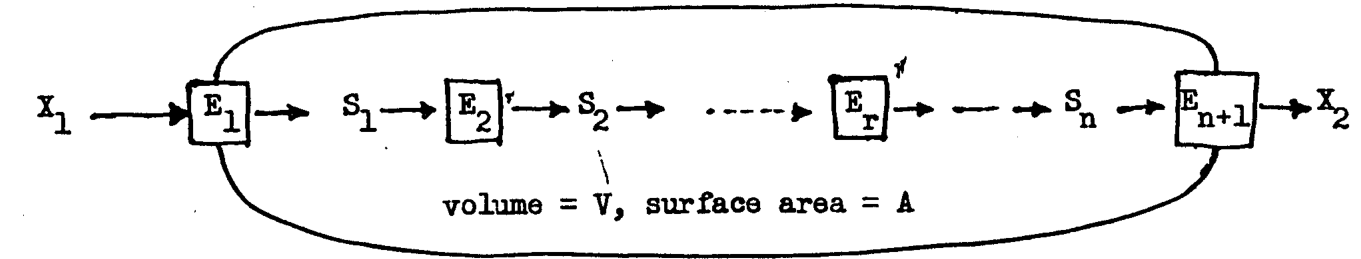
\includegraphics[max width=\textwidth]{figure1_chain}
\end{center}

By `linear' is meant that the rate-expressions for the separate reactions of type, $A \rightleftarrows B$, are of the form.
%
\begin{equation}
f = \rho(A-B / K) \tag{1.13a}
\label{eqn:113a}
\end{equation}
%
where $f$ is the net flux from A to $B$ per unit quantity of enzyme, $K$ is the equilibrium constant for the reaction and $\rho$ is a kinetic constant. In fact every enzyme catalyzed reaction will have a non-linear rate expression, since saturation can always occur and (1.13a) is merely an approximation which holds provided the concentrations, $A$ and $B$, remain within certain limits. For example the simple non linear rate-expression for a unimolecular reaction mentioned in the introduction was of the form
%
\begin{equation}
f = \frac{\vecur{T}}{\vecur{M}}\left(A - \frac{B}{K}\right) /\left(1 + \frac{A}{\vecur{M}} + \frac{B}{\vecul{M}}\right) \tag{1.13b}
\label{eqn:113b}
\end{equation}
%

This approximates to the linear form (1.13a) provided $A \ll \vecur{M}$ and $B \ll \vecul{M}$, the constant $\rho$ then equals $\frac{\vecur{T}}{\vecur{M}}$.

In the diagram $E_{1}, E_{2}, \ldots$ are used both as `names' for the enzymes and also to refer to their concentrations, similarly for the metabolites $S_{1}, S_{2}, \ldots$. Provided that the metabolites are well mixed the enzymes can be distributed non uniformly in the volume in which case $E_{r}$ refers to the average concentration. Transport enzymes such as $\mathrm{E}_{1}, \mathrm{E}_{\mathrm{n+l}}$ will have to be situated, not necessarily uniformly, on the surface but their `linear' rate expressions will be formally similar. Even if transport is non-enzymic and therefore depends on the surface area, A, there will be an effective `concentration of area', $A/V$, which will be genetically (parametrically) defined and will play a similar role to enzyme concentration.

Considering the rate of change of the 1st metabolite in the whole volume
%
$$
\frac{d\left(V_{X} S_{1}\right)}{dt} = \left(E_{1} \times V\right) \rho_{1}\left(X_{1} - \frac{S_{1}}{K_{1}}\right) - \left(E_{2} \cdot V\right) \rho_{2}\left(S_{1} - \frac{S_{2}}{K_{2}}\right)
$$
%
or
%
\begin{equation}
\dot{S}_{1} = E_{1} \rho_{1}\left(\mathrm{X}_{1}-\frac{\mathrm{S}_{1}}{\mathrm{K}_{1}}\right)-\mathrm{E}_{2} \rho_{2}\left(\mathrm{S}_{1}-\frac{\mathrm{S}_{2}}{\mathrm{K}_{2}}\right)-\left(\frac{1}{\mathrm{V}}\dot{V}\right) \mathrm{S}_{1}
\label{eqn:114}
\end{equation}
%
The products $E_{r} \rho_{r}$ etc. can be written as $v_{r}$. Where $v_{r}$ means the activity of the rth enzyme per unit volume of the system when the substrate has unit and the product zero concentration. Writing $F_{1}, F_{2}$, as, the net fluxs/unit volume of the system and remembering that $\left(\frac{1}{\olsi{V}}\dot{V}\right)$ is zero, the set of dynamical function $\varphi_{1}, \ldots, \varphi_{\mathrm{n}}$ are given by
%
\begin{equation}
\begin{aligned}
 \varphi_{1} &=\dot{S}_{1}=v_{1}\left(\mathrm{X}_{1}-\frac{\mathrm{S}_{1}}{\mathrm{K}_{1}}\right)- v_{2}\left(\mathrm{S}_{1}-\frac{\mathrm{S}_{2}}{\mathrm{K}_{2}}\right)=\mathrm{F}_{1}-\mathrm{F}_{2} \\[4pt]
\varphi_{2}&=\dot{\mathrm{S}}_{2}=v_{2}\left(\mathrm{S}_{1}-\frac{\mathrm{S}_{2}}{\mathrm{K}_{2}}\right)-v_{3}\left(\mathrm{S}_{2}-\frac{\mathrm{S}_{3}}{\mathrm{K}_{3}}\right)=\mathrm{F}_{2}-\mathrm{F}_{3} \\
& \vdots
\\
 \varphi_{n}&=\dot{S}_{n}=v_{n}\left(\mathrm{S}_{n-1}-\frac{\mathrm{S}_{\mathrm{n}}}{\mathrm{K}_{n}}\right)-v_{n+1}\left(\mathrm{S}_{\mathrm{n}}-\frac{\mathrm{X}_{2}}{\mathrm{K}_{n+1}}\right)=\mathrm{F}_{n}-\mathrm{F}_{n-1}
\end{aligned} \tag{1.15a}
%\label{eqn:115}
\end{equation}
%
The conditions, $\varphi_{i}=0$, for a stationary solution give rise to a set of $n$ linear simultaneous equations for the $n$ unknown stationary values $\olsi{S}_{i}$ and these equations could be solved; because of their simple structure, by straightforward algebraic elimination. However, they will be treated in a more general way both to illustrate the methods just described and to facilitate extension later to the "non-linear straight chain" where algebraic elimination is not possible.

The equations (1.15a) are equivalent to the `band matrix' equation

\begin{center}
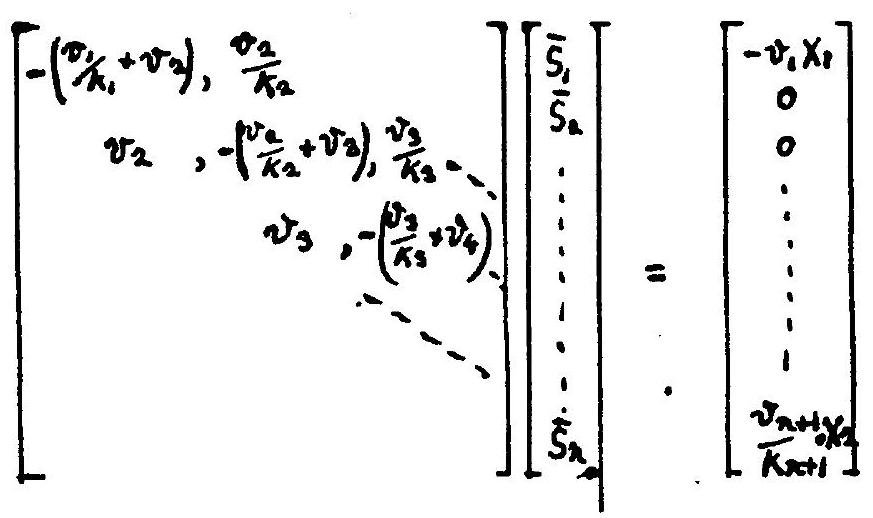
\includegraphics[scale=0.35]{2023_01_30_a974a42f7b7381f3f940g-041}  \mbox{\hspace{15pt} (1.15b)}
\end{center}
\stepcounter{equation}
\stepcounter{equation}
Hence there is just one S.S. which furthermore turns out to be completely stable in the sense that the dynamics of the approach to this S.S. is a sum of decaying exponentials, (Denbigh, Hicks and Page, 1947). This latter property arises because the dynamical matrix $[D]$, which in this case is identical to the band matrix above, possesses special features. Since these features are of a general nature they will be dealt with later. in this chapter.

However, inverting the matrix gives little insight into how the $\olsi{S}_{i}$, or indeed important measures of the system such as the pathway flux, $\olsi{F}$, depend on the parameters.. This can be shown as follows. At the S.S. all the separate fluxes are equal to the pathway flux so that:
%
\begin{equation}
\begin{aligned}
\olsi{F}=\olsi{F}_{1} &= v_{1}\left(\olsi{X}_{1}-\frac{S_{1}}{\olsi{K}_{1}}\right) \\[4pt]
\olsi{F}=\olsi{F}_{2} &= v_{2}\left(S_{1}-\frac{S_{2}}{K_{2}}\right) \\[4pt]
\olsi{F}=\olsi{F}_{n+1} &= v_{n+1}\left(S_{n}-\frac{X_{2}}{K_{n+1}}\right)
\end{aligned}
\label{eqn:116}
\end{equation}
%
If $\olsi{F}$ is the correct pathway flux there are $n+1$ linear equations to solve for only $n$ unknowns, $\olsi{S}_{1} \ldots \olsi{S}_{n}$. This means that the coefficients must be linearly dependent and implies that their $(n+1)$ determinant is zero.
%

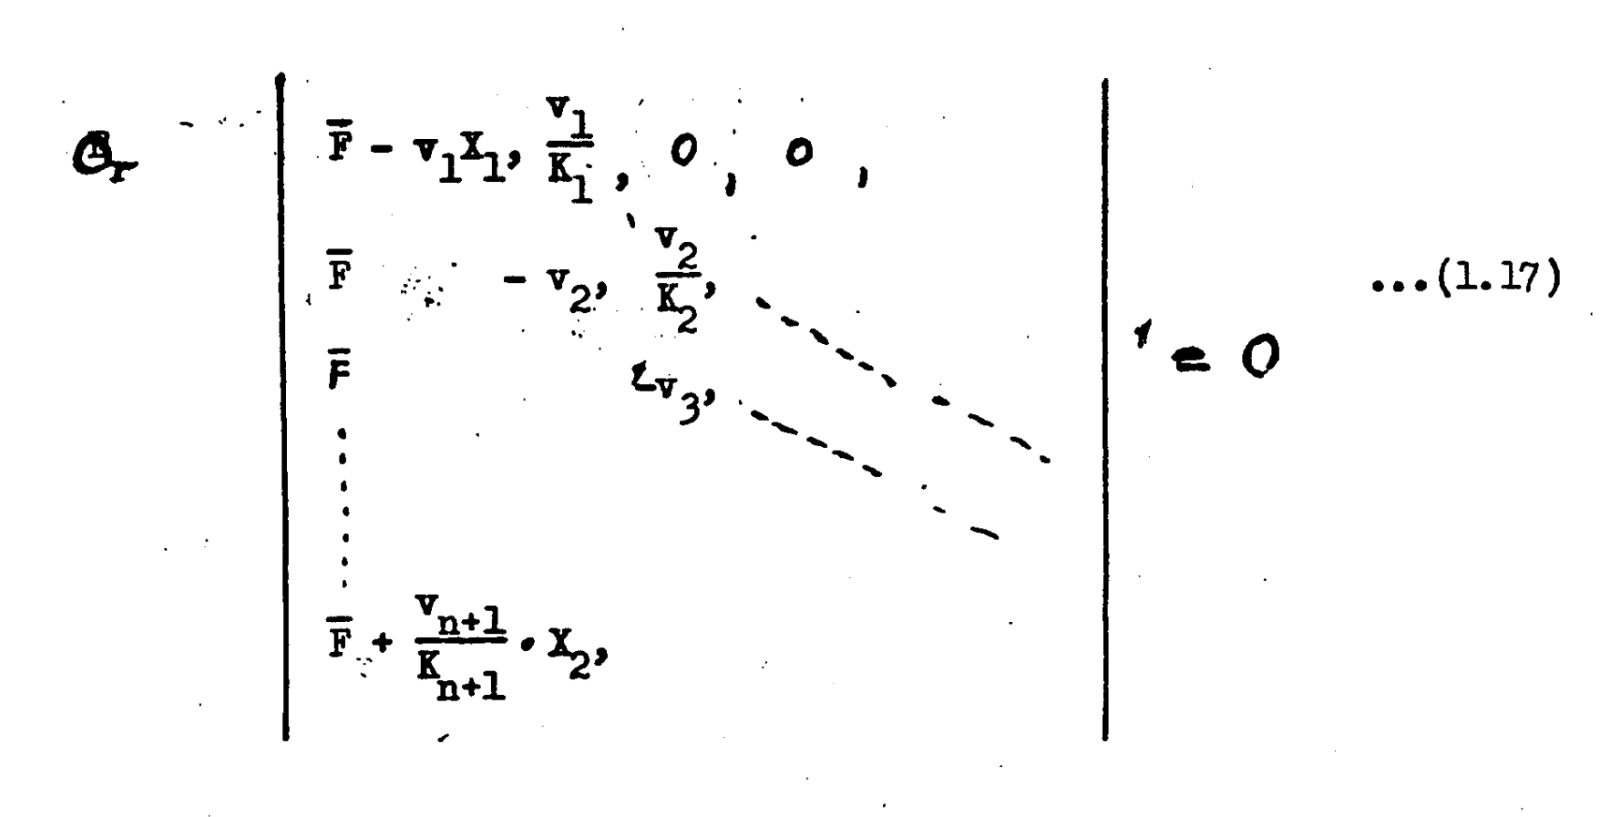
\includegraphics[scale=0.5]{figure1_17.png}

%
Since $\olsi{F}$ occurs only in the 1st column this is a simple linear equation in $\olsi{\mathrm{F}}$ and when expanded gives on simplifying this yields
%
\stepcounter{equation}

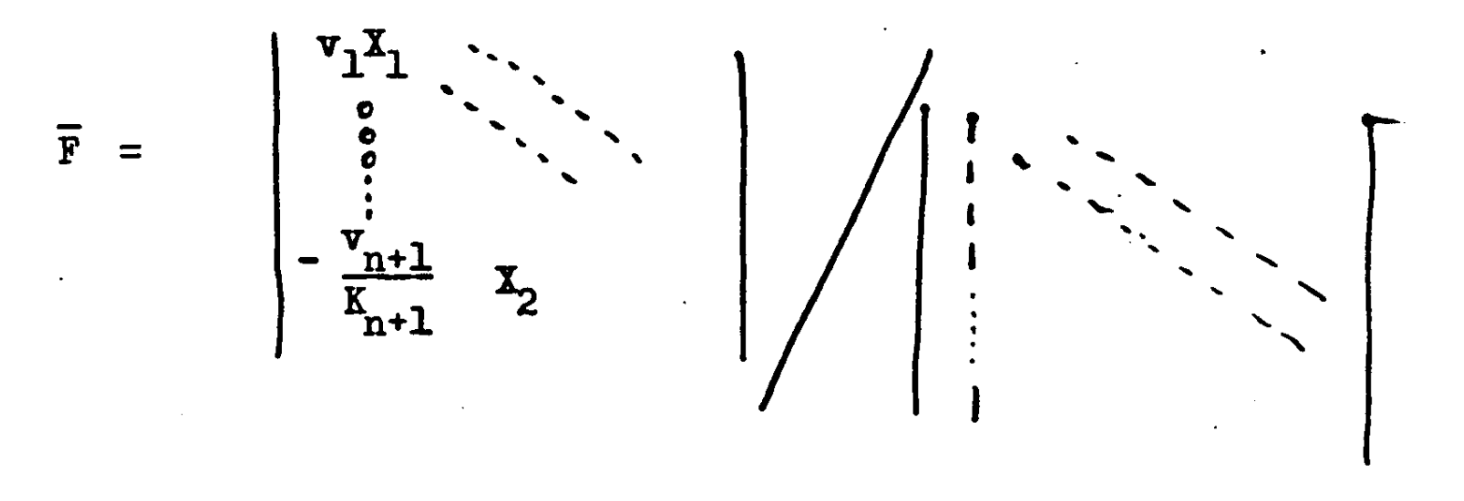
\includegraphics[scale=0.55]{figure1_17a.png}
%
%\centerline{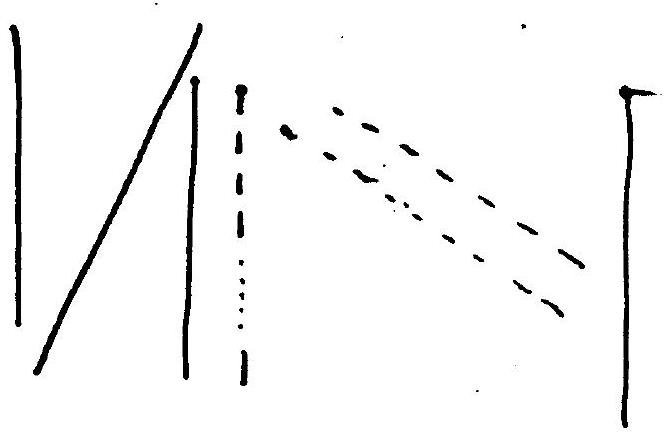
\includegraphics[scale=0.3]{2023_01_30_a974a42f7b7381f3f940g-043}}
$$
\overline{\mathrm{F}} = \mathrm{X}_1-\frac{\mathrm{X}_2}{\mathrm{K}_1 \cdot \mathrm{K}_2 \cdots \mathrm{K}_{n+1}} \bigg/
\left(\frac{1}{v_1} + \frac{1}{\mathrm{K}_1 v_2} + \frac{1}{\mathrm{K}_1 \mathrm{K}_2 v_3} +
\cdots \frac{1}{\mathrm{K}_1 \mathrm{K}_2 \cdots \mathrm{K}_n v_{n+1}}\right)  \mbox{(1.18)} $$

Having found $\olsi{F}$ it is a simple matter to compute $S_{1}, S_{2}$ etc. using successively the equations of (1.16).

\section{The sensitivity coefficient}

The relation (1.18), allows us to see explicitly exactly how the measure $\olsi{F}$ depends on the parameters $v_{1}, v_{2}, \cdots$ In this case the flux controlling effect of the separate enzymes in, the pathway will be measured by the set of sensitivity coefficients $C_{v_{i}}^{\olsi{F}}$ and an expression can be found, employing the usual definition.

Thus
%
\stepcounter{equation}
\begin{equation}
\begin{aligned}
C_{v_{i}}^{\olsi{F}} &= \frac{v_{i}}{\olsi{F}} \cdot \frac{\partial \olsi{F}}{\partial v_{i}}=v_{i} \frac{\partial \log (\olsi{F})}{\partial v_{i}} \\
&=v_{i} \left(-1 \bigg/ \frac{1}{v_{1}}+\frac{1}{K_{1} v_{2}} \cdots \cdots\right) -\frac{1}{K_{1} K_{2} \ldots v_{i}^{2}} \\
C_{v_{i}}^{\olsi{F}} &=\frac{1}{K_{1} \ldots K_{i-1} v_{i}} \bigg/\left(\frac{1}{v_{1}}+\frac{1}{K_{1} v_{2}}+\ldots \ldots\right)
\end{aligned}
\label{eqn:119}
\end{equation}

The two properties, $0 < C_{v_i}^F < 1$ and $\displaystyle \sum_{i=1..n} C_{v_i}^F = 1$ immediately follow.

Since \eqref{eqn:119} is of the form, $C^{F}_{v_{i}} = \frac{a_{i}}{\sum a_{i}}$, it is clear that the separate coefficients are all positive and less than unity and that in addition the sum of the separate coefficients is unity.

This leads to the important result that if any enzyme is found to have a control coefficient of approximately one it must be the controlling or `throttling' enzyme in the sequence since the sum of all the other control coefficients will be small. For example a system having four reactions all with $K_{E}=1$, three catalysed by enzymes of activity $v$ and one of them, say the 2nd, by an enzyme of activity $v/9$ would be expected to have rate-control mainly from the second enzyme.

Broadly how strong this effect is can be seen from substituting in \eqref{eqn:119},
%
$$
C^{\olsi{F}}_{v_2} = \frac{1}{v/9} \bigg/ \frac{1}{v} + \frac{1}{v/9} + \frac{1}{v} + \frac{1}{v} = \frac{9}{12} = 75 \%
$$
%
Thus of the total $100 \%$ control available $75 \%$ is `owned' by the 2nd enzyme and $8.3 \%$ by each of the others.

In a real situation, we may wish to know which is the limiting enzyme in a sequence but find it inconvenient or impossible to estimate the response of $\olsi{F}$ to a modulation in $v_{i}$ for several enzymes. In these circumstances it would be useful if some other `measure' were diagnostic of rate control. Such a `diagnostic' might be related to the pattern of the pools. Thus for the previous example, the pool levels are shown in the following diagram if $X_{1}$ is taken as 100 and $X_{2}$ as zero.

\begin{center}
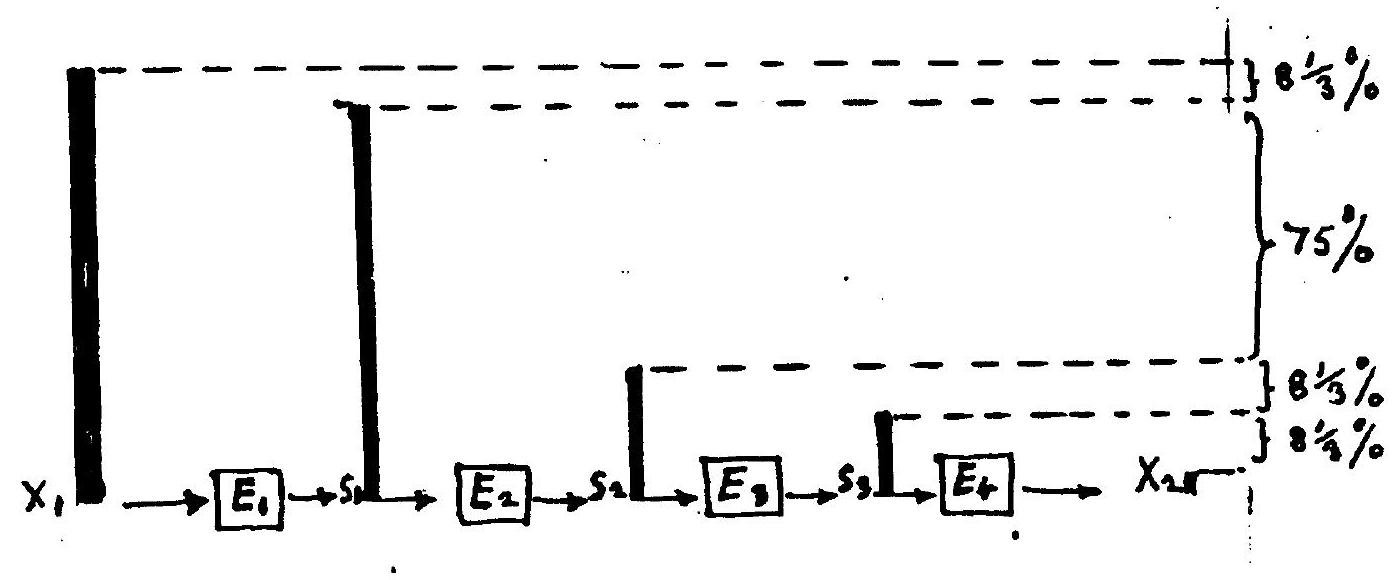
\includegraphics[max width=\textwidth]{2023_01_30_a974a42f7b7381f3f940g-045}
\end{center}

In this case the main drop is indeed across the 2nd enzyme and in fact it is true that the difference between pools on either side of an enzyme is a measure of its relative rate controlling effect. Will this be so for arbitrary $X_{1} X_{2}$ and when $K_{1} K_{2}$ etc are not unity?

From \eqref{eqn:119}
%
$$
 \quad C_{v_{i}}^{\olsi{F}} \propto \frac{1}{K_{1} K_{2} \ldots v_{i}}
$$
%
and also the set of equation \eqref{eqn:116}  can be written as
$$
\frac{1}{v_{1}} = \frac{X_{1}}{\olsi{F}} \cdot\left(\frac{X_{1}}{X_{1}}-\frac{S_{1}}{K_{1} X_{1}}\right) = \frac{X_{1}}{\olsi{F}} Q_{1}
$$

$$\frac{1}{\mathrm{K}_1 v_2} = \frac{\mathrm{X}_1}{\olsi{F}} \left(\frac{\mathrm{S}_1}{\mathrm{K}_1 \mathrm{X}_1}-\frac{\mathrm{S}_2}{\mathrm{K}_1 \mathrm{K}_2 \mathrm{X}_1}\right) = \frac{\mathrm{X}_1}{\olsi{F}}  {Q}_2$$

so that the factors $Q_{1}, Q_{2}...$ are proportional to the coefficients of the respective enzymes. The meaning of these factors is apparent when it is noted that $K_{1} X_{1}, K_{1} K_{2} X_{1}, \ldots$ are the values $, S_{1}^{*}, S_{2}^{*}$, which $S_{1}, S_{2}$ would take if the flux in the pathway were blocked and equilibrium were established along the chain. The factors $Q_{1}, Q_{2}, \ldots$ etc are then just

$$\left(1-\frac{\olsi{S}_{1}}{S_{1}^{*}}\right), \left(\frac{\olsi{S}_{1}}{S_{1}^{*}} - \frac{\olsi{S}_{2}}{S_{2}^{*}}\right), \ldots \mbox{etc.} $$

In principle then an experiment could be done which first observed the levels of $\olsi{S}_{1}, \olsi{S}_{2}$ etc. then observed the values $S_{1}^{*}, S_{2}^{*}$, which resulted from blocking the pathway. Scaling the $\olsi{S}_{i}$ by their own equilibrium values, $S_{i}^{*}$, would result in a set of numbers, the difference between successive pairs yielding $Q_{1}, Q_{2} \cdots$. One advantage of such a diagnostic would be that it only involves ratios of concentrations of single pools and hence does not depend on the metabolites being uniformly extractable.

\section{The network}

The system just dealt with at some length had a number of relatively simple properties. Thus it was completely stable, possessed only one stationary state, the sum of rate control over the enzymes was unity and finally the pool pattern gave a simple `diagnostic' of which step was exerting control. In addition there was a simple expression for the pathway flux as a function of the parameters. It will be of interest to see to what extent these properties are retained as more realistic features are introduced into unimolecular systems. Thus we fan consider a more general \underline{network} of such linear unimolecular reactions, or consider the case where saturation effects are incorporated into the rate expressions.

The general network of linear unimolecular reactions allows for more than two external metabolites and also for any amount of branching and convergence of pathways. A typical network containing nine enzymes is shown below and exemplifies the possible features.
%
\begin{center}
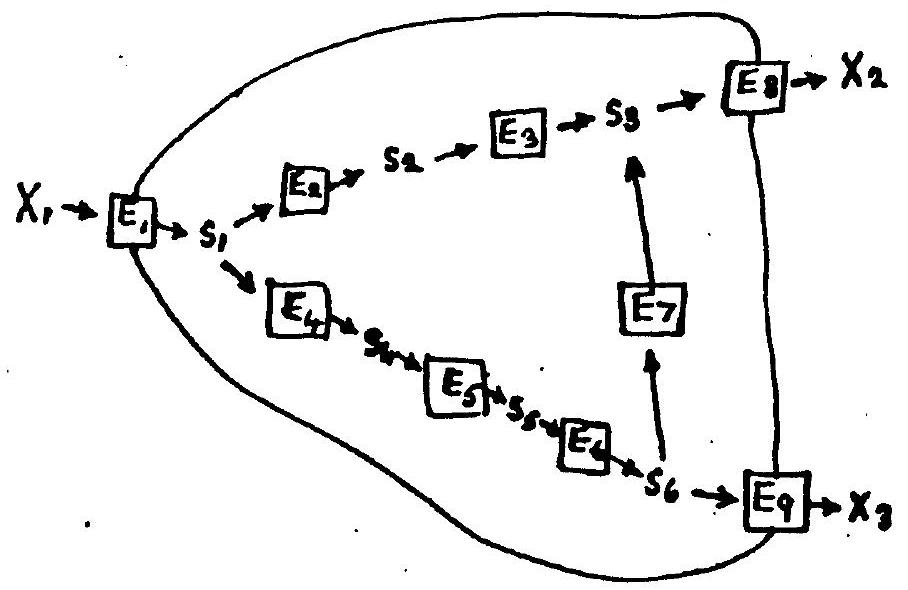
\includegraphics[scale=0.3]{2023_01_30_a974a42f7b7381f3f940g-047}
\end{center}
%
Of particular interest is that it is now possible to have a cycle of reactions in the sense that molecules leaving $S_{1}$, along one path may return on another.

The general network is allowed for in the scheme below which shows the exchange between any two arbitrary internal metabolites $S_i, S_j$ and also between any internal metabolite $S_1$ and external $X_q$. The net flux, used previously, is here considered as being made up of the +ve and -ve parts of the linear rate expression (1.13a).

\begin{center}
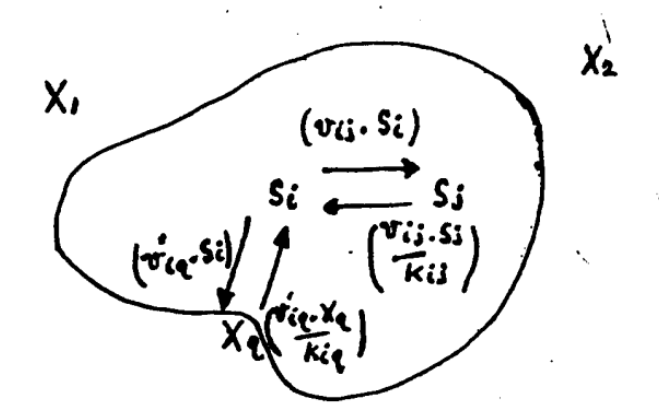
\includegraphics[scale=0.7]{figure1_system.png}
\end{center}

The constant $K_{i, j}$ is the equilibrium constant for the reaction $S_i \rightleftharpoons S_j$ and is defined as $\left(\frac{S_j}{S_i}\right)$ eq. If all the reactions are truly unimolecular then, when more than one route exists between two metabolites, the product of the $\mathrm{K}_{\mathrm{E}}$s must be the same for both routes (Levis, 1925). For example in the nine enzyme network above $\mathrm{K}_{1,2} \cdot \mathrm{K}_{2,3}=\mathrm{K}_{1,4} \cdot \mathrm{K}_{4,5} \cdot \mathrm{K}_{5,6} \cdot$ K$_{6,3}$. The dynamical equations for the general network are written down in a similar way to those for the straight chain and are

\begin{equation}
\varphi_i=\dot{S}_i=-\sum_{\mbox{all} j\neq i} v_{ij} \left(S_i-\frac{S_j}{K_{i,j}}\right)-\sum_q v_{iq}^{\prime}\left(S_i-\frac{X_q}{K_{iq}^{\prime}}\right)
\label{eqn:120}
\end{equation}

Since the network is truly unimolecular there will be a unique product of equilibrium constants between $\mathrm{X}_1$ (say) and any other metabolite, $S_i$ or $X_{q}$ Let these products be denoted by $\eta_i$ and $\eta^{\prime}_q$.

\section{The electrical analogue}

It will now be shown that if each $S_{1}$ and $X_{q}$ is scaled by its appropriate $\eta$ the equations (1.20) will assume a particularly simple form from which certain observations follow. These scaled variables are $\theta_{i}=\frac{S_{i}}{\eta_{i}}$ and $\theta_{q}^{\prime}=\frac{X_{q}}{\eta^{\prime}_q}$ and the equations (1.20) may be grouped as follows:
%
$$
\eta_{i} \times \left(\frac{\dot{S}_{i}}{\eta_{i}}\right) = -\sum v_{ij} \cdot \eta_{i}\left(\frac{S_{i}}{\eta_{i}}-\frac{S_{i}}{K_{i,j} \eta_{i}}\right)- \sum \cdots
$$
%
then noting that, by definition, $X_{i,j} \eta_{i}=\eta_{j}$ we have
%
$$
\eta_{i} \dot{\theta}_{i}=-\sum \eta_{i} v_{ij}\left(\theta_{i}-\theta_{j}\right)- \sum \eta_{i}^{\prime} v_{iq}^{\prime}\left(\theta_{i}-\theta_{q}^{\prime}\right)
$$
%
finally, introducing $\rho_{ij}=\eta_{i} v_{ij}$ and noting that this quantity is symmetric, since
%
$$
\rho_{ij}=\eta_{i} v_{ij}=\eta_{i} K_{ij} \cdot \frac{v_{i j}}{K_{i j}}=\eta_{j} \cdot v_{ji}=\rho_{ji}
$$
%
The equations (1.20) assume the form
%
\begin{equation}
\eta_{i} \dot{\theta}_{i}=-\sum_{j \neq i} \rho_{i j}\left(\theta_{i}-\theta_{j}\right)-\sum_{q} \rho_{iq}^{'}\left(\theta_{i} - \theta_{q}^{i}\right)
\label{eqn:121}
\end{equation}
%
A set of interconnected earthed capacitors will be described by exactly the same set of.equations when some of the capacitor is are connected via conductances $\rho_{i q}^{\prime}$ to fixed voltages, $\theta_{q}^{\prime}$, the ith capacitor having capacitance $\eta_{i}$ and the conductance between the ith and $j$th capacitor being $\rho_{i j}$ Thus the general enzyme network shown previously is, in this sense, exactly equivalent to the general electric network following.

\begin{center}
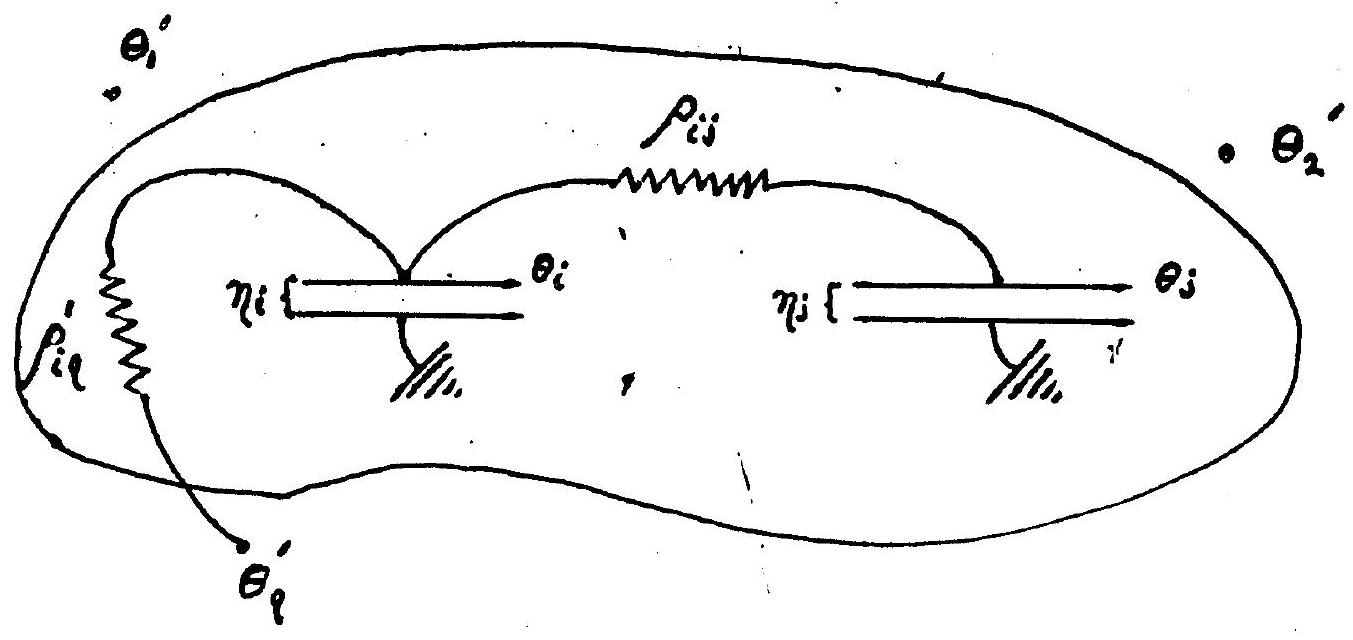
\includegraphics[max width=\textwidth]{2023_01_30_a974a42f7b7381f3f940g-050}
\end{center}

The rule of equivalence is that at the ith node of the chemical network should be placed a capacitor whose value, $\eta_{i}$, is the product of the equilibrium constants between $X_{1}$ and the node, and that each enzyme having activity $v_{ij}$ radiating from this node should be placed by a conductance of value $\eta_{i} v_{ij}$ Then the fluxes in the enzyme network will be numerically identical with the currents in the electrical system, and the voltages $\theta_{i}$ at the nodes will be related to the metabolic pools by $S_{i}=\eta_{i} \cdot \theta_{i}$. There is no confusion about the values to be given conductances, according to which node they are calculated from, since $\eta_{i} v_{ij}=\eta_{j} v_{ji}$. When interest is centred on the stationary state the values assigned to the capacitors are unimportant and the equivalent system is merely the network of conductances.

This equivalence principle makes clear why the straight chain of reactions had simple properties, since no matter how many conductances are placed in series they still behave as one conductance which can be found by a simple rule for compounding them. For more complicated networks the stationary fluxes can easily be found by applying the known Kirchoff laws.

As an example the general branched pathway will be considered. To start with consider a system with only three reactions and where $\mathrm{X}_{1}$ is converted via a branching system into $\mathrm{X}_{2}$ and $\mathrm{X}_{3}$. The two equivalent systems are shown below

%$X_{1} \stackrel{v_{1}}{\stackrel{\sim}{v_{1} / X_{0}}} S_{1}$

\begin{center}
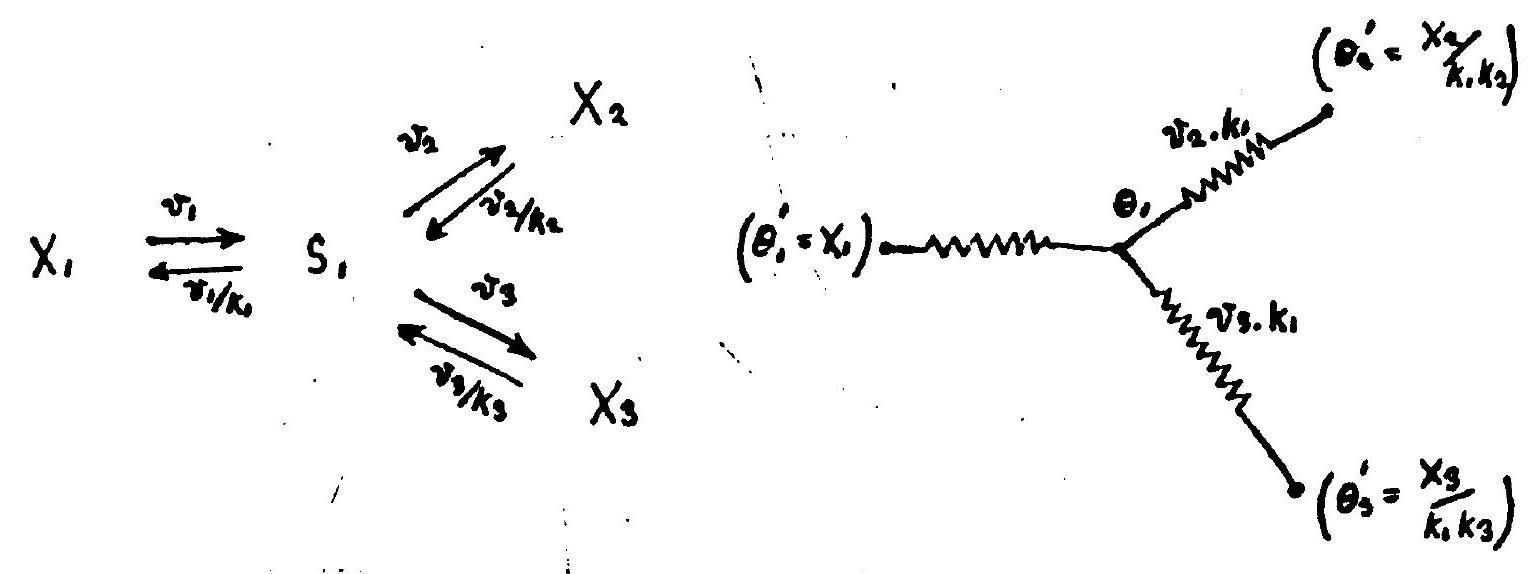
\includegraphics[max width=\textwidth]{2023_01_30_a974a42f7b7381f3f940g-051}
\end{center}

%\begin{center}
%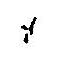
\includegraphics[max width=\textwidth]{2023_01_30_a974a42f7b7381f3f940g-051(1)}
%\end{center}

The fixed voltages $\theta^{\prime}$ are found from the fixed chemical concentration by the appropriate scaling. The sum of the current leaving the branch point must be zero, so that

$$
\begin{aligned}
& \left(\theta_{1}-\mathrm{X}_{1}\right)+\left(\theta_{1}-\frac{\mathrm{X}_{2}}{\mathrm{K}_{1} \mathrm{K}_{2}}\right) \cdot v_{2} \mathrm{K}_{1} + \left(\theta_{1}-\frac{\mathrm{X}_{3}}{\mathrm{K}_{1} \mathrm{K}_{3}}\right) \cdot v_{3} \cdot \mathrm{K}_{1} = 0 \\[5pt]
& \text { or } \theta_{1} = \frac{X_{1} v_{1} + X_{2} v_{2} \bigg/ K_{2} + X_{3} v_{3} \bigg/ K_{3}}{v_{1} + v_{2} K_{1} + v_{3} K_{1}}
\end{aligned}
$$
%
hence, for example, the flux in the 1st enzyme being numerically identical to the electrical current is
%
$$
\overline{F}_{1}=v_{1}\left(X_{1}-\theta_{1}\right) = v_{1}\left(\frac{X_{1}\left(v_{2} K_{1}+v_{3} K_{1}\right)-X_{2} v_{2} \bigg/ K_{2}-X_{3} v_{3} \bigg/ K_{3}}{v_{1}+K_{1} v_{2}+K_{1} v_{3}} \right)
$$
%
If each pathway had contained several enzymes it would only have been necessary to replace the conductances $v_{1}, \mathrm{K}_{1} v_{2}, \mathrm{K}_{1} v_{3}$ by the overall conductance possessed by, each pathway. These are found by the rule for summing a sequence of conductors which is that for example the four conductances where

\begin{center}
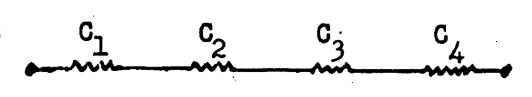
\includegraphics[scale=0.8]{figure1_conductance.png}
\end{center}

behave as one conductance $C$ where:
%
$$
1/C= 1/C_{1} + 1/C_{2} + 1/C_{3} + 1/C_{4}
$$
%
When applied to a straight chain this immediately yields an equivalent single conductance of value
%
$$
C = 1 \bigg/ \frac{1}{v_{1}} + \frac{1}{K_{1} v_{2}}+\frac{1}{\mathrm{K}_{1} \mathrm{K}_{2} v_{3}} + \cdots
$$
%
an expression which was involved in the flux through a straight chain studied earlier.

\section{Stability}

The property of dynamical stability is still possessed by the general network of reactions just discussed and this can be proved in a very general way. Thus in the equivalent electrical network the rate of dissipation of energy in a single conductance is current $x$ voltage or $\rho_{ij}\left(\theta_{i}-\theta_{j}\right) \times\left(\theta_{i}-\theta_{j}\right)$ and the total rate of dissipation, $L_{,}$in the network is given by
%
\begin{equation}
L = \sum \rho_{ij}\left(\theta_{i}-\theta_{j}\right)^{2} + \sum \rho_{iq}^{\prime}\left(\theta_{i}-\theta_{q}^{\prime}\right)^{2}
\label{eqn:122}
\end{equation}
%
where the summation is over all conductors. It can easily be verified that
%
$$
\begin{aligned}
& \frac{\partial L}{\partial \theta_{1}}=2 \sum_{j \neq i} \rho_{i j}\left(\theta_{i}-\theta_{j}\right)+2 \sum \dot{\rho}_{iq}^{\prime}\left(\theta_{i}-\theta_{q}^{\prime}\right) \\
\end{aligned}
$$
or using \eqref{eqn:121}
%
\begin{equation}
\frac{\partial_{L}}{\partial \theta_{i}}=-2 \eta_{i} \dot{\theta}_{i}
\label{eqn:123}
\end{equation}
%
Now when the system is in motion
%
$$
\dot{L} = \sum \left(\frac{\partial L}{\partial \theta_{i}}\right) \cdot \dot{\theta}_{i}
$$
%
or from \eqref{eqn:123}
%
\begin{equation}
\dot{L} = -2 \sum \eta_{i}\left(\dot{\theta}_{i}\right)^{2}
\label{eqn:124}
\end{equation}
%
Inspection of \eqref{eqn:122} and \eqref{eqn:124} shows that throughout any motion $L \geqslant 0$ and $\dot{L}<0$. Which implies that the dynamical system, when, released from any initial condition, can only move towards a stable stationary state. The results just established, equivalence to an electrical network and complete stability, apply to networks of linear unimolecular reactions and depend on the property that the product of equilibrium constants along different paths connecting the same metabolites is identical. This condition will also be satisfied in many networks of interest, which include `pseudo unimolecular' reactions provided these do not appear within any `cycle' of reactions.

By a `pseudo unimolecular' reaction is meant, for example, one of the form $A+B \rightleftarrows C+D$ but where $B$ and $D$. can be considered as parameters $B^{\prime}$ and $D^{\prime}$, that is as constant concentrations external to the dynamical system. In this case the true thermodynamic eq. constant $K_{E}=\left(\frac{C \times D^{\prime}}{A_{\times} B^{\prime}}\right)$ but since $B^{\prime}$, and $D^{\prime}$ are constant these will be an effective equilibrium constant $K_{E}$ for the pseudo-unimolecular reaction $A \rightleftarrows$ C. This constant is given by $K_{E}^{\prime}=K_{E} \times \frac{B^{\prime}}{D^{\prime}}$ and clearly is subject to no thermodynamic constraint. $\frac{B^{\prime}}{D^{\prime}}{ }^{\prime}$ being set at arbitrary level.

The \underline{general pseudo-unimolecular network} having linear rate expressions has no equivalent electrical network and correspondingly does not have the same simple solution and stability properties. However, even for this case there is a stability property which might be said to depend on the `conservation of molecules', found in all unimolecular systems. Thus in the equations \eqref{eqn:120}, for the general system, if the molar concentrations are measured as differences $S_{i}^{\prime}$ from the stationary values $\olsi{S}_{i}$ the equation of motion will be
%
\begin{equation}
\left[\begin{array}{c}
\dot{S}_1^{\prime} \\[5pt]
\dot{S}_2^{\prime} \\
\vdots \\
\end{array}\right]=\left[\begin{array}{l}
D
\end{array}\right]\left[\begin{array}{c}
S_1^{\prime} \\[5pt]
S_2^{\prime} \\
\vdots \\
\end{array}\right]
\label{eqn:125}
\end{equation}
%
where, for this linear system, the dynamical matrix $D$ has constant elements. A simple argument shows that these elements satisfy certain conditions. Suppose that all $S_{i}^{\prime}=0$ except one, say $S_{3}^{\prime}$, which is +ve then clearly, from the metabolic diagram and a consideration of the rate expression, $\dot{S}_{3}^{\prime}$ must be -ve and all other $\dot{S}_{i}^{\prime}$, re or zero, depending on whether they receive molecules from $\mathrm{S}_{3}$ or not. Furthermore, since all molecules leaving $S_{3}$ must arrive at other intermediate metabolites or leave the system, the sum of $\dot{S}_{3}^{\prime}$ and all other $\dot{S}_{i}^{\prime}$ must be $\leq 0$. Hence the matrix $D$ will have the form

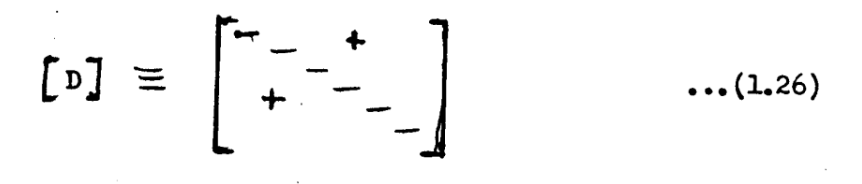
\includegraphics[scale=0.55]{figure1_1_26}

That is, -ve diagonal and all other elements +ve or zero. In addition D will satisfy the condition that in each column the sum of the elements is less than or equal to zero. These are sufficient conditions (HEARON, 1963) to ensure the stability of the system in the sense that although complex eigenvalues may occur their real parts will be -ve. This means that such systems may have a tendency to oscillate but that these oscillations will always be decaying.

In the case of networks not containing pseudo-unimolecular reactions within loops, it is always possible by suitably scaling the dynamical variables to symmetrise the matrix D, since this corresponds to the condition $\rho_{ij} = \rho_{ji}$ in (1.21). This further property of symmetrisability is sufficient to ensure that all eigenvalues of D are real (Hearon, 1963), so that such systems move towards their stationary solutions as a sum of decaying exponential terms. The straight chain mentioned earlier, whether it is truly unimolecular or not, is an example of this.

An example of a network, in which we are interested, containing potentially oscillatory cycles is the arginine cycle, indicated below.

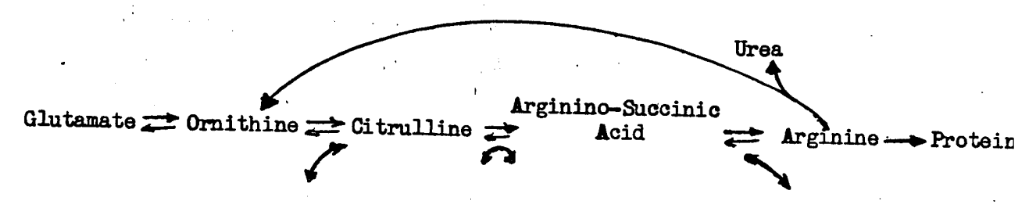
\includegraphics[scale=0.7]{figure1_argpathway}

Here several of the reactions within the cycle involve other metabolites. Even if these are treated as constant, so that the system is unimolecular, the fact that the product of equilibrium constants around different sides of the loop is not the same cannot be ignored. However, the general property proved above indicates that when the arginine system is approximated by linear rate-expression it will have just one stable solution, possibly arrived at via decaying oscillations.

The situation when the rate expressions for reactions in a unimolecular network are non-linear is of interest. In this case there will still be a set of equations similar to (1.25) for movement about the stationary state, but they will only apply for small disturbances from the $\olsi{S}_i$ and the elements of D will become the $\left[\frac{\partial \varphi_i}{\partial S_j}\right]_{S_j=\olsi{S}_{j}}$, discussed earlier.

However, the argument that (D) had the general form (1.26) and that its columns satisfied the required inequalities assumed only `conservation of molecules', which of course is still true, and that the rate expressions were restricted to have certain properties. The required properties are that they should involve only their own substrates and products and that when the level of a metabolite is increased its net rate of removal by a given enzyme should respond positively in the algebraic sense. Such properties are fairly general and will certainly be possessed by the simple rate-expression of (1.13b) allowing for saturation. Thus it is still possible to state, subject to this restriction, that the general network of non-linear unimolecular reactions will be stable, with decaying oscillations, in the neighbourhood of a stationary solution. For example if the arginine cycle were represented by nonlinear rate-expressions it would still be stable. However for true unimolecular networks with cycles the introduction of a saturable rate expression within a cycle could alter the type of stable dynamical behaviour, since the matrix [D] will no longer be symmetrisable.

With the introduction of non-linear rate expressions it becomes possible to represent `end product inhibition' and this is indicated below.

\begin{center}
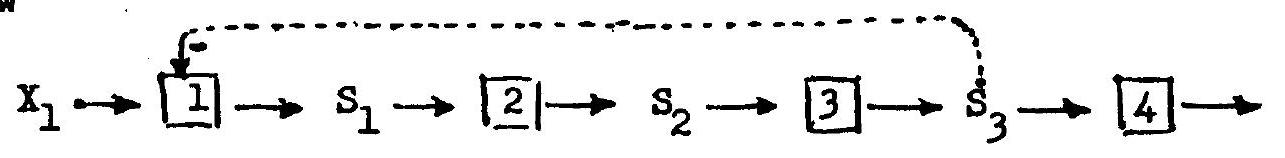
\includegraphics[max width=\textwidth]{2023_01_30_a974a42f7b7381f3f940g-057}
\end{center}

The rate expression for the 1st reaction, in this case, involves $\mathrm{S}_{3}$. Under these circumstances the system may become unstable since there are now off-diagonal -ve elements in [D]. Increasing the `strength' of the feedback corresponds to increasing the magnitude of the off-diagonal element and at some point the previously stable system will become unstable. However, because of the inherent stability of the initial system, a considerable feedback signal can be tolerated without instability. The stability of such systems has been treated subject to a number of simplifying assumptions (Walter, 1969).

\section{Nonlinear systems}

Turning now to the problem of locating the stationary state for a non linear unimolecular system it is clear that there will be no simple algebraic method since we now have a set of simultaneous non linear equations. The simplest case to consider is that of a straight chain of reactions where each enzyme has a rate-expression of the form (1.13b). This situation corresponds to the sequence of linear reactions discussed on p. 16 except that the fluxes per unit volume of the system become
%
\stepcounter{equation}
\begin{equation}
F_{i} = \frac{v_{i}}{\vecur{M_{i}}}\left(S_{i-1} - \frac{S_{i}}{K_{i}}\right) \big/ \left(1 + \frac{S_{i-1}}{\vecur{M_{i}}} + \frac{S_{i}}{\vecul{M_i}}\right)
\label{eqn:127}
\end{equation}
%
Where $v_{i}$ is now the maximum velocity of the ith enzyme in the direction $S_{i-1} \rightarrow S_{i}$ and for unit volume of the system $v_{i}$ will be proportional to the concentration $E_{i}$ of the enzyme. The constants $\vecur{M_{i}}$ and $\vecul{M_{i}}$ are the appropriate Michaelis constants and $K_{i}$ is the `effective' equilibrium constant for the step. Once again there are $n+1$ linear equations in $S_{1}, S_{2} \cdots S_{n}$ expressing the fact that at the stationary state the $n+1$ separate fluxes are all equal to the pathway flux $\olsi{F}$ These are obtained by multiplying up the denominator in expressions of the form (1.27) and yield.

%\section{$37 \cdot$}
\begin{center}
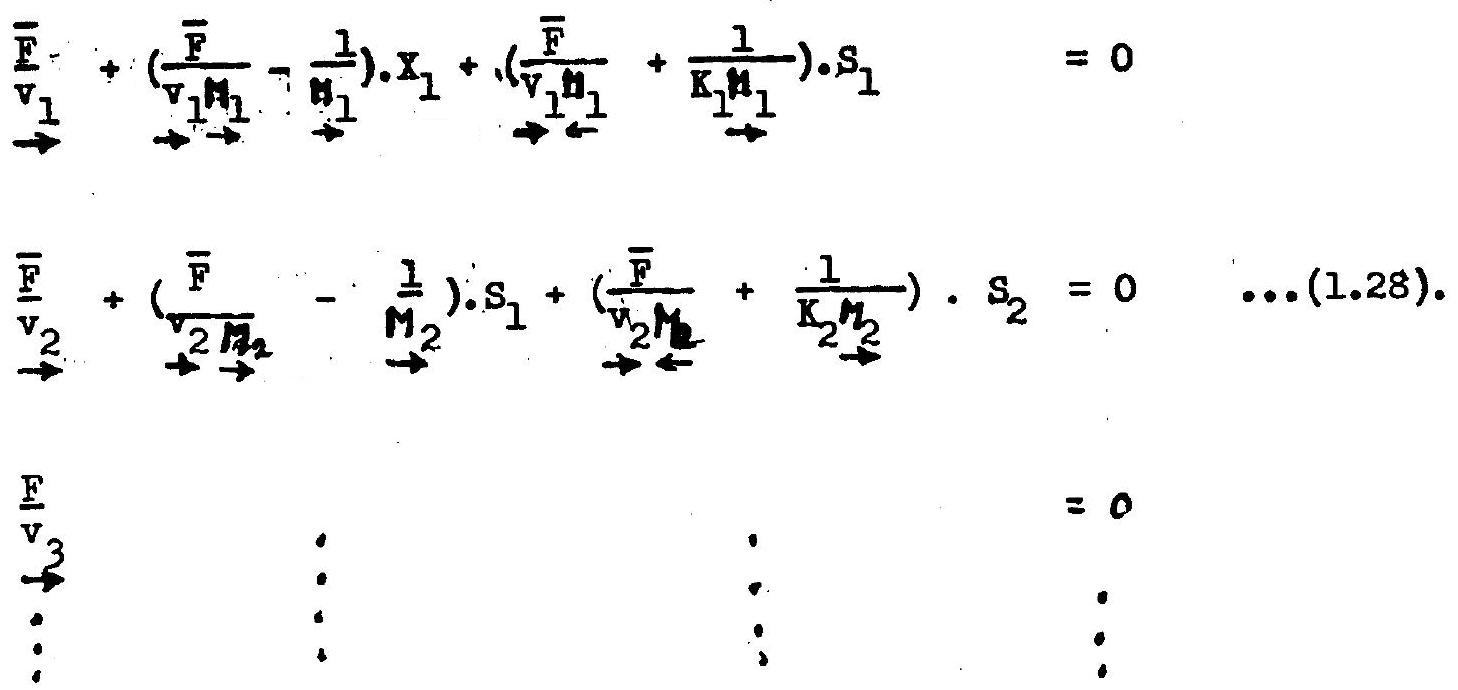
\includegraphics[max width=\textwidth]{2023_01_30_a974a42f7b7381f3f940g-059}
\end{center}

As before there are $(n+1)$ equations to determine only $n$ unknowns that the determinant of the coefficients must be zero or,

\begin{center}
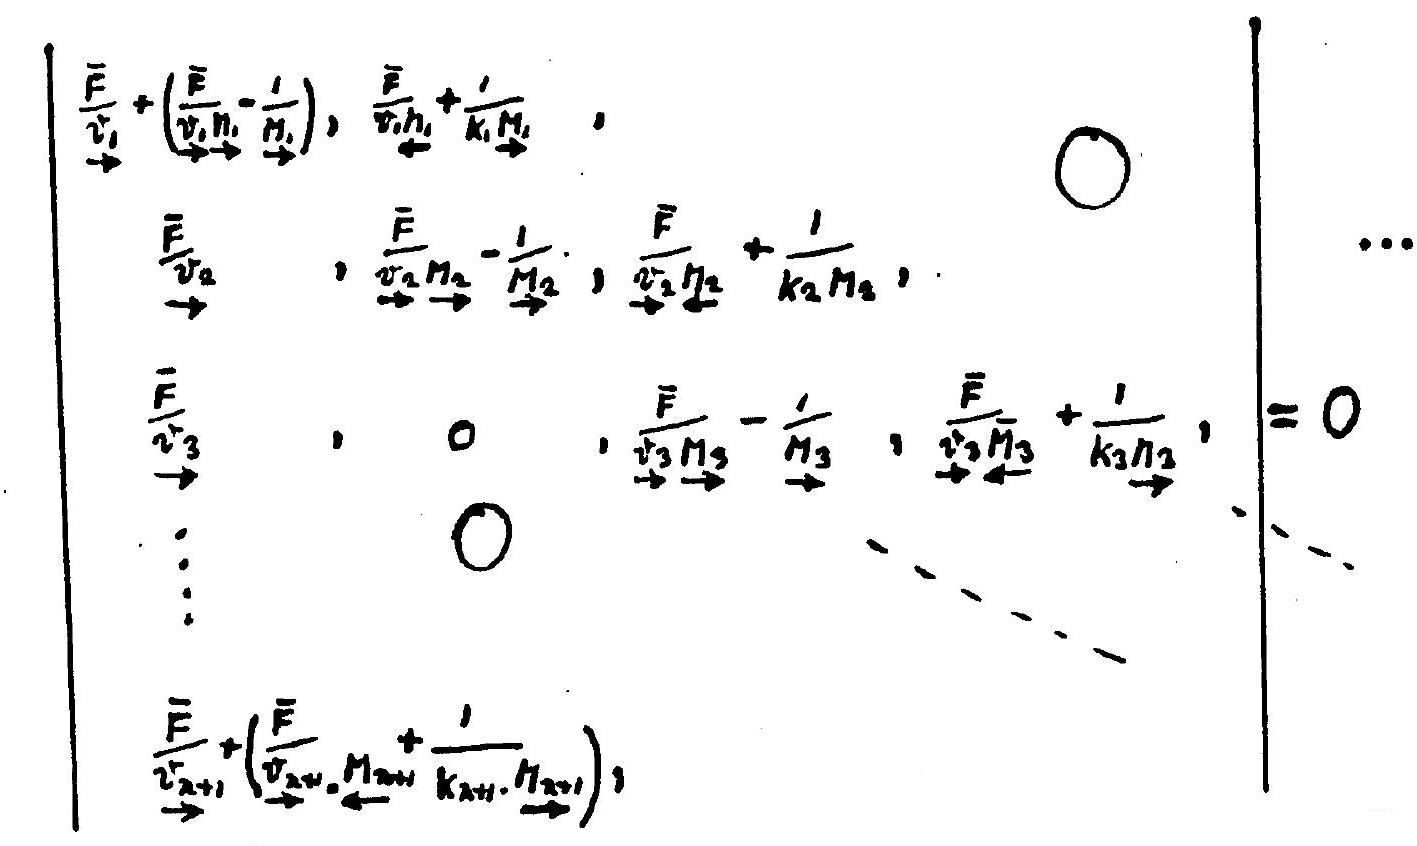
\includegraphics[max width=\textwidth]{2023_01_30_a974a42f7b7381f3f940g-059(1)}
\end{center}

The pathway flux, $\olsi{F}$, must satisfy the determinental equation, but $\olsi{F}$ now occurs in all elements of the determinant whereas formerly, in the linear case, it was present only in the first column. Consequently the equation of which $\olsi{F}$ is a solution is now a polynomial in $\olsi{F}$ of order $n+1$. Thus for two enzymes $\olsi{F}$ is one of the roots of a quadratic equation and for 10 enzymes it is one of the 10 roots of the 10th order equation. In fact it turns out that in this system there is never more than one $\olsi{F}$ satisfying the condition that all $\olsi{S}_i$ should be real and +ve. One consequence of $\olsi{F}$ being the solution of a high order equation is that there will no longer be an explicit formula, corresponding to (1.18) of the linear case, giving $\olsi{F}$ in terms of the parameters. Nor is it any longer the case that the overall action of a sequence of enzymes is equivalent to one enzyme. It appears then that when non-linear rate expressions are introduced, even in the simple case of a straight chain, there is no alternative but to study possible to investigate the `non-linear straight chain' problem algebraically with respect to the question of `diagnosing' from the pool pattern which steps in the chain are rate controlling. This question will be returned to in CH II, at the moment it will be show that even though there is no explicit expression for the flux it is still true that $\sum \mathrm{C}_{v_i}^{\olsi{F}}=1$. This can easily be seen by noting that in the functional relationship existing between $\olsi{F}$ and $v_{i}$.
%
$$
\olsi{F} = \olsi{F}\left(v_1, v_2, \ldots v_{2+1}\right)
$$
Thus simultaneous changes in the $v_i$ will cause a small change in $\olsi{F}$ according to
%
\stepcounter{equation}\stepcounter{equation}
\begin{equation}
\delta \olsi{F}= \sum \frac{\partial \olsi{F}}{\partial v_{i}} \cdot \delta v_{i}
\label{eqn:130}
\end{equation}
%
Now inspection of the determinant (1.28) shows that if all $v_{i}$ are increased by the same factor $(1+a)$ then $\olsi{F}(1+a)$ will be the new solution. So that changes $\alpha v_{1}, \alpha v_{2}, \dots$ produce a change $\alpha \olsi{F}$ in the flux. When $\alpha$ is small this can be substituted in (1.30) and

$$ \alpha \olsi{F} = \sum_i \frac{\partial \olsi{F}}{\partial v_i} \cdot \alpha v_i $$
%
or
%
\begin{equation}
1 = \sum \frac{v_i}{\olsi{F}} \cdot \frac{\partial \olsi{F}}{\partial v_i} = \sum C_{v_i}^{\olsi{F}} 
\label{eqn:131}
\end{equation}
%
Thus it appears that the summation property of rate control coefficients, originally proved for the linear case, may be a fairly general one.
